
%%%%%%%%%%%%%%%%%%%%%%% file typeinst.tex %%%%%%%%%%%%%%%%%%%%%%%%%
%
% This is the LaTeX source for the instructions to authors using
% the LaTeX document class 'llncs.cls' for contributions to
% the Lecture Notes in Computer Sciences series.
% http://www.springer.com/lncs       Springer Heidelberg 2006/05/04
%
% It may be used as a template for your own input - copy it
% to a new file with a new name and use it as the basis
% for your article.
%
% NB: the document class 'llncs' has its own and detailed documentation, see
% ftp://ftp.springer.de/data/pubftp/pub/tex/latex/llncs/latex2e/llncsdoc.pdf
%
%%%%%%%%%%%%%%%%%%%%%%%%%%%%%%%%%%%%%%%%%%%%%%%%%%%%%%%%%%%%%%%%%%%


\documentclass[runningheads,a4paper]{llncs}
\let\proof\relax
\let\endproof\relax
\usepackage{amsthm}

\usepackage{ amssymb}
\usepackage{amsmath}

\setcounter{tocdepth}{3}
\usepackage{graphicx}

\theoremstyle{definition}
%\newtheorem{definition}{Definition}[section]
\theoremstyle{plain}
%\newtheorem{theorem}{Theorem}

%\newtheorem{lemma}[theorem]{Lemma}

%\newtheorem{claim}{Claim}

\usepackage{subcaption}
\captionsetup{compatibility=false}
\graphicspath{ {images/} } 

\usepackage{booktabs}
\usepackage{multirow}

\usepackage{url}
\urldef{\mailsa}\path|{alfred.hofmann, ursula.barth, ingrid.haas, frank.holzwarth,|
\urldef{\mailsb}\path|anna.kramer, leonie.kunz, christine.reiss, nicole.sator,|
\urldef{\mailsc}\path|erika.siebert-cole, peter.strasser, lncs}@springer.com|    
\newcommand{\keywords}[1]{\par\addvspace\baselineskip
\noindent\keywordname\enspace\ignorespaces#1}

\begin{document}

\mainmatter  % start of an individual contribution

% first the title is needed
\title{Lecture Notes in Computer Science:\\Authors' Instructions
for the Preparation\\of Camera-Ready
Contributions\\to LNCS/LNAI/LNBI Proceedings}

% a short form should be given in case it is too long for the running head
\titlerunning{Lecture Notes in Computer Science: Authors' Instructions}

% the name(s) of the author(s) follow(s) next
%
% NB: Chinese authors should write their first names(s) in front of
% their surnames. This ensures that the names appear correctly in
% the running heads and the author index.
%
\author{Alfred Hofmann%
\thanks{}%
\and Ursula Barth\and Ingrid Haas\and Frank Holzwarth\and\\
Anna Kramer\and Leonie Kunz\and Christine Rei\ss\and\\
Nicole Sator\and Erika Siebert-Cole\and Peter Stra\ss er}
%
\authorrunning{Lecture Notes in Computer Science: Authors' Instructions}
% (feature abused for this document to repeat the title also on left hand pages)

% the affiliations are given next; don't give your e-mail address
% unless you accept that it will be published
\institute{Springer-Verlag, Computer Science Editorial,\\
Tiergartenstr. 17, 69121 Heidelberg, Germany\\
\mailsa\\
\mailsb\\
\mailsc\\
\url{http://www.springer.com/lncs}}

%
% NB: a more complex sample for affiliations and the mapping to the
% corresponding authors can be found in the file "llncs.dem"
% (search for the string "\mainmatter" where a contribution starts).
% "llncs.dem" accompanies the document class "llncs.cls".
%

\toctitle{Lecture Notes in Computer Science}
\tocauthor{Authors' Instructions}
\maketitle


\begin{abstract}
The abstract should summarize the contents of the paper and should
contain at least 70 and at most 150 words. It should be written using the
\emph{abstract} environment.
\keywords{We would like to encourage you to list your keywords within
the abstract section}
\end{abstract}
\section{Introduction}
In these decades, reachability of verification has caught much significant attention. However, the main difficulty is that computation of state-space explosion grows exponentially as the order number of state variables increasing. To overcome this challenge, abstraction techniques are often used in verification on complex systems. The process is to study an over-approximation abstraction, which simplifies a system with allowing more behaviors. Therefore, the original system is safe from the error states if the abstraction is safe from the error states.\\
\section{Related work}
Model order reduction (MOR) can obtain a lower-dimensional system that captures the essential features of an original high-dimensional system. Solving problem in a lower dimension, one can get the result more efficiently. The technique has been applied commonly in control theory \cite{Lall02asubspace},\cite{doi:10.1080/00207170410001713448}, which investigated reducing the computation complexity of large-dimensional dynamical systems, while preserving the input-output behavior to their best of the ability. In addition, MOR methods to address the lidnear system are well established, such as balanced truncation (BT) \cite{Lall02asubspace}, Krylov Methods (KMs) \cite{SALIMBAHRAMI2006385}, which keep the most controllable and observable states. In reality, physical systems usually are the nonlinear system, which should be more primarily considered, but still only a few number of methods for nonlinear systems exist. proper orthogonal decomposition (POD) and trajectory piecewise linearization (TPWL) are the most popular methods. POD calculates the singular value decomposition of snapshot matrix generated from trajectories at certain instances of time \cite{Pinnau2008}. The basic concept of TPWL is to transform a full-order nonlinear system into a combination of a set of reduced-order linear models by hybridization of a nonlinear system \cite{REWIENSKI2006426}.\\
Verification of linear systems and hybrid systems with MOR technique has been explored in Ref \cite{1386733},\cite{Han2006},\cite{Tran2017}. Ref \cite{1386733} developed a a reachability approximation procedure with BT reduction method, and they analyzed the error bound derived from reducing order for verification of high-dimensional linear systems. Furthermore, authors in \cite{Tran2017} compared different methods of estimating error bound in several high-dimensional linear systems. To avoind large estimated error bound, initial conditions should be close to the zeor point, which is one of main concernings in their studies. Also, Ref.\cite{Han2006} applied KMs to a class of reachability analysis problems of large-scale affine systems. However, for nonlinear systems, it is hard to estimate a conservative error that accounts for model order reduction. In this paper, we discussed verification on nonlinear systems with POD method and analyzed the unsafety reachability with a statistical error bound.\\
The remainder of the paper is organized as follows. Section \ref{Preliminaries} describes the reachability problems considered in our studies. Section \ref{POD} outlines how to construct a reduced-order model with POD algorithm and a statistical error bound. Section \ref{specification} and Section \ref{verification process} demonstrates the procedure of unsafety verification of reduced abstraction. We present and evaluate the result of verification with MOR in Section \ref{case studies}. Finally, Section \ref{conclusion} summarizes our works in this paper.


\section{ Preliminaries} \label{Preliminaries}
In this section, we will introduce the definition of the reachability problem, the projection-based model and the unsafety transformation through this paper. First, a continuous nonlinear system $S_n$ is defined by: 
\begin{equation}
\dot{x}(t)=f(x(t))+Bu(t), \quad x \in \mathbf{R^n} \\ \label{xode} 
\end{equation}
where $f \in \mathbf{R^n}$, $B \in \mathbf{R^{n\times m}}$, and $u(t) \in \mathbf{R^m}$ is the control input. 
Given an initial state $x_0 \in X_0$, $\psi(t)$ is the trajectory of x evolves with Eq.(\ref{xode}) over a finite time horizon$ [0, t_f]$. For a reachability problem, we analyze whether the sets $\psi(t)$ with all initial states $x_0 \in X_0$ reach any unsafe state $y \in X_f(S_n)$. Formally, if $R_{[0,t_f]}(S_n,X_0) \cap X_f(S_n)=\emptyset $, where the reachable sets $R_{[0,t_f]}(S_n,X_0 ) = \left\{ {y=\psi(t,x) \, |\, t\in [0,t_f], x\in X_0}\right\}$. 

Next, we will formalize an abstraction of the reduced-order system, which is used to verify the properites of the full-order system.

\begin{definition}{Reduced-order abstraction}
The k-dimensional system $S_k$ with $k<n$ described by $\dot{z}=f_r (z(t))$, where $z(t) \in \mathbf{R^k}$, $z(0) \in Z_0$, $f_r \in \mathbf{R^k}$, and it aprroximates the dynamics of $S_n$. We call $S_k$ as a reduced-order abstraction of  $S_n$. 
\end{definition}
\begin{definition}{Unsafe specification Transformation}
A unsafe specification transformation is to generate the corresponding unsafe region $X_f(S_k)$ for the reduced-order abstraction $S_k$ from the original unsafe region $X_f(S_n)$ such that guarantees the relation as bellows:\\
\begin{equation}
X_f(S_k)\cap R_{[0,t_f]}(S_k,Z_0 )=\emptyset \Rightarrow  X_f(S_n) \cap R_{[0,t_f]}(S_n,X_0)=\emptyset  \label{Unsafe_Tran}
\end{equation}
\end{definition}
    
\section{Proper orthogonal decomposition} \label{POD}
\subsection{Process of constructing reduced model}
To find a reduced model for large-dimensional systems, proper orthogonal decomposition (POD) is applicable to non-linear system, and it preserves the overall non-linear dynamics. The POD projection-based method is based on singular value decomposition (SVD) of the sampled dynamical-data collected over a time range \cite{Pinnau2008},\cite{Stadlmayr2015}. Data from the simulation of original models are used to generate the basis onto which the original states are projected, and it aims to form a approximation system with smaller-dimensional which retains as many important features as possible. The scheme for constructing the projection basis and the reduced model can be summarized in the following steps:\\
(1) Randomly select an initial state $x_0 \in X_0$ and simulate trajectory from $t=0$ to $t_f= N$ N times, and further construct the set of snapshot matrix $\mathrm{X=[X_1, X_2,...,X_N]} \in \mathbf{R^{n \times Nl}} $ with $\mathrm{ X_i} =[x_i (t_0),x_i (t_1),...,x_i (t_f)] \in \mathbf{R^{n\times l}} $ for $i=0 \backsim N.$\\
(2) Construct the global reduced subspace by performing a SVD on the snapshots $ \mathrm{X}= UDV^T$,\\
where $U=[U_1 U_2 ...U_n] \in \mathbf{R^{n\times n}}$ is a left-singular matrix, $V \in \mathbf{R^{Nl\times Nl}}$ is a right-sigular matrix, and $D=diag(\sigma_1, \sigma_2, ...,\sigma_n)$, where $\sigma_1\geq \sigma_2\geq ...\geq \sigma_n$ are the sigular values of $\mathrm{X}$.  \\
(3) The POD basis is selected by the $k (k<<n)$ left-singular vectors of $\mathrm{X}$corresponding to the $k$ largest singular values, and the projection operator $U_r=[U_1 U_2 ... U_k] $ is defined. 
The POD basis is the optimal basis that minimizes the least squares error of snapshots over set of orthogonal basis of size $k$, ie.\cite{LIANG2002527},\\
\[
\min_{\Phi \in \mathbf{R^{n\times k}}}\parallel\mathrm{X}-\Phi \Phi^{T}\mathrm{X}\parallel_2^2,  \quad s.t. \quad \Phi^T  \Phi =\mathrm{I},
\]
where $\mathrm{I}$ is an identity matrix, and the POD basis give optimal value as $\sum_{i=k+1}^n=\sigma_i^2$. Therefore, the quantitative guidance for choosing proper reduced size $k$ is provided by the singular values of snapshots matrix. Typically, we can select the value $k$ such that $\frac{\sum_{i=k+1}^n}{\sum_{i=1}^n} < \kappa$ with a user-specified tolerance $\kappa$ (often being 0.01$\%$ or smaller \cite{Pinnau2008}).      
 \\
(4) Project the original space into reduced subspace, and the dynamic equation in the reduced-order subspace becomes
\[
\dot{z}(t)=g(z(t))+B_k u(t), \quad  z_0=U_r^T x, \quad    z\in \mathbf{R^k} \\ \label{xrode} 
\]
where $g(z(t))=U_r^T f(U_r z(t))$ can obtained by symbolic substitution, $B_k=U_r^T B$.
\
\subsection{Statistical error bound} 
For the specific initial condition that generated the data used in constructing the reduced model, its error bound of the approximated solution of the original system can be obtained. However, we are interested at the error bound for all $x_0 \in X_0$ when solving verification problem. To overcome that problem, it can be considered as the resulting error caused by the perturbations of the initial conditions. Ref\cite{Homescu05errorestimation} provides an approach on combining the small sample statistical condition estimation (SCE) method with error estimation using the adjoint method. The general idea is demonstrated here.\\

Based on SCE method proposed in Ref\cite{Kenney:1994:SSC:180322.180327}, for any vector $e \in \mathbf{R^n}$, if a set of orthogonal vectors $\{\upsilon_1, \upsilon_2,...,\upsilon_q\}$ is uniformly and randomly generated from a unit sphere $\{\upsilon \in \mathbf{R^n} \mid || \upsilon||=1\}$, then the expected value of norm of the component of $e$ in the span $\{\upsilon_1, \upsilon_2,...,\upsilon_q\}$ directions is\\
\[
E(\sqrt{|\upsilon^T_1 e|^2+|\upsilon^T_2 e|^2+...+|\upsilon^T_q e|^2})=\frac{W_n}{W_q}||e||,
\]  
where $W_n$ is \textit{Wallis factor} defined as\\
\[W_1=1,\quad W_n=\left\{
\begin{array}{lll}
\frac{1\cdot3\cdot\cdot\cdot(n-2)}{2\cdot4\cdot\cdot\cdot(n-1)}      &      & \mbox{n odd}\\
\frac{2}{\pi}\frac{2\cdot4\cdot\cdot\cdot(n-2)}{1\cdot3\cdot\cdot\cdot(n-1)}     &      & \mbox{n even}
\end{array} \right.\]
and approximated with $W_n \approx \sqrt{2/(\pi(n-1/2))}$. Therefore, $\bar{e}(q)\equiv\frac{W_q}{W_n}\sqrt{|\upsilon^T_1 e|^2+|\upsilon^T_2 e|^2+...+|\upsilon^T_q e|^2}$ is an subspace condition estimator of the norm $||e||$ with $q$-th order accurate \cite{Homescu05errorestimation}, i.e., given a factor of size $\gamma>1$, the probability that the estimator $\bar{e}(q)$ lies within the factor of $\gamma$ of $||e||$ has a relative error $\epsilon$ proportional to $\gamma^{-q}$ as belows,
\begin{equation}
\mathrm{Pr}\left( \frac{||e|| }{\gamma}\leq \bar{e}(q)\leq \gamma||e||\right)\approx 1-O(\frac{1}{\gamma^q}),
\end{equation}
and more details are shown in Ref.\cite{Kenney:1994:SSC:180322.180327}.\\

Reminding that the POD-reduced model can be constructed with specific initial condition $x_0$ from simulation, we have its exact solution $\bar{x}(t)$ and approximated solution $\tilde{x}(t)$ for $t=[0,t_f]$. Therefore, the error $||e^0(t)||=||\bar{x}(t)-\tilde{x}(t)||$ can be obtained. Moreover, we need to analyze the error in the case that some perturbation in the initial conditions of the original model. Let us consider the perturbed ODE equation and the approximated POD based equation written as,
\begin{align}
\dot{x^p}(t)&=f(x^p,t), \quad x^p(0)=\bar{x}_0 +\delta \bar{x}_0,\\
\dot{\tilde{x}}^p(t)&=P f(\tilde{x}^p,t), \quad \tilde{x}^p(0)=P (\bar{x}_0 +\delta \bar{x}_0),
\end{align}
with $P=U_r U_r^T \in \mathbf{R^{n \times n}}$. The error $E(t_f)=\tilde{x_f}^p(t)-x^p(t_f)$ can be estimated as following.\\
First, we redefine another error term $\Delta'=E(t_f)-e^0(t_f)$ to estimate, which makes $||E(t_f)||$ bounded by 
\begin{equation}
||E(t_f)||\leq ||e^0(t_f)||+||\Delta'|| \label{error}
\end{equation} 
To analyze the norm error $||\Delta'||$, we split it into two components: $||\Delta'_\perp||$, which is orthogonal to the POD-reduced subspace, and $||\Delta'_\parallel||$, which is parallel to the subspace.
According to Ref.\cite{Homescu05errorestimation}, we can estimate $||\Delta'_\perp||\approx \frac{W_q}{W_n}\sqrt{\sum_{j=1}^q |\lambda_j^T (0)\delta \bar{x}_0|^2}$ by using SCE method and solving the adjoint system defined by $\frac{d\lambda_j(t)}{dt}=-J^T(\bar{x},t)\lambda_j(t)$ with $\lambda_j(t_f)=(I-P) \upsilon_j$, where $J$ is the Jacobian evaluted at $\bar{x}$ and $\upsilon_j$ is a random vector uniformly selected from a unit sphere $S_{n-1}$. Also, it has shown that $||\Delta'_\parallel(t)||\approx 0$ to a first order approximateion for any $t>0$. Thus, from Eq.(\ref{error}) the statistical error bound becomes
\begin{equation}
||\delta_s||\equiv||e^0(t_f)||+\kappa_p ||\delta \bar{x}_0||, \quad \mbox{with}\quad \kappa_p=\frac{W_q}{W_n}\sqrt{\sum_{j=1}^q ||\lambda_j^T (0)||^2}
\end{equation}
As a result, \textit{a-priori} statistical error bound within specific region of initial condition $X_0$ can be obtained before having to solve the original system and the corresponding reduced system with all initial condition $\{x_0 \in X_0\}$  

\section{Transforming unsafe specification in reduced-order abstraction}  \label{specification}
To perform verification on a reduced-order abstraction, we need to transform the unsafe specification $X_f$ from those states of a full-order system to those of a reduced-order system. Ref.\cite{Tran2017} have discussed the transforming of safe and unsafe specifications described by convex polytopes and ellipsoids, and we consider the specification as convex polytopes in flow* tool \cite{6987596}. In the following, the transformed specification is presented in detail. At the beginning, it assumes that the unsafety specification of the full-order system is forming as:    
\begin{equation}
X_f(S_n)=\{x \in \mathbf{ R^n} \, |\, Ax> b\}\\\label{unsafe_n} 
\end{equation}
where $A=\left[ a_{ij}\right] \in \mathbf{ R^{q\times n}}$ and $b=\left[ b_{i}\right] \in \mathbf{ R^q}$. \\
\begin{lemma}
Given $X_f(S_n)$ defined by Eq.(\ref{unsafe_n}),  then $X_f(S_k)$ is defined as belows.\\
\begin{equation}
X_f(S_k)=\{z \in \mathbf{ R^k} \, |\, A_r z > \bar{b}\}
\end{equation}
where $A_r=A U_r$ and $\bar{b}=b-\bigtriangleup$ with $\bigtriangleup=[\bigtriangleup_i] \in \mathbf{ R^q},$ $\bigtriangleup_i=\sum_{j=1}^n  a_{ij} \delta_j$,  is a n-dimensional error bound $\delta \in \mathbf{ R^n}$.
\end{lemma}
\begin{proof}
Substitute the definition of $x \approx U_r z$ with the error bound $\delta$ into constraints Eq.(\ref{unsafe_n}), it gives $\sum_{k=1}^{n} a_{ik}U_r(k,j) z_j - |a_{ij}|\delta_j < a_{ij} x_j<\sum_{k=1}^{n} a_{ik}U_r(k,j) z_j + |a_{ij}|\delta_j $. Thus, we have $ A_r z- \bigtriangleup<A x<A_r z+ \bigtriangleup$, and further it gives $ A_r z- \bigtriangleup-b<A x-b<A_r z+ \bigtriangleup-b$. To satisfy Eq.(\ref{Unsafe_Tran}), we have the relaxation constraint $A_r z>b-\bigtriangleup$ to contain the region $Ax>b$.
\end{proof}
Noted that in our study on verification, we use the statistical error bound $|\delta_s|$ introduced previously. $\bigtriangleup_i=|\delta_s| \sum_{j=1}^n  a_{ij}$ is applied. 
%For performing falsification, we choose $\bigtriangleup=0$.  
Geometrically, the unsafe specification of the original systems is included in the transformed unsafe region of in reduced-order abstraction with a $(1-\epsilon)$ confidence.
\section{Unsafety verification with a reduced abstraction}  \label{verification process}
First, we demonstrate a stastical verification technique. 
\begin{lemma}
Given a continuous nonlinear system $S_n$, if its reduced-order abstraction $S_k$ with a $(1-\epsilon)$ confidence error bound $|\delta_s|$ doesn't reach the transformed unsafe region, it guarantees that the original system $S_n$ is safe with $(1-\epsilon)$ confidence.
\end{lemma}
 \begin{proof}
According to the definition of the reduced abstraction, for any trajectory of $S_n$ with $x_0 \in X_0$, there exists a corresponding trajectory of $S_k$, which is at most $|\delta_s|$ far from the original trajectory with $(1-\epsilon)$ confidence. Besides, the transformed unsafe specification of the abstraction described by previous section including the unsafe specification of the original system is designed to satisfy Eq.(\ref{Unsafe_Tran}). That implies that if all corresponding trajectory of $S_k$ do not reach the relaxation unsafe region in the subspace, all trajectory of $S_n$ won't reach the unsafe region in the full-order space with $(1-\epsilon)$ confidence.
 \end{proof}
On the other side, if the verification of the $k$-order reduced model claims that it is reachable to the unsafe states, we repeat the same algorithm to perform verification in the reduced abstraction, whose dimension is increased by 1 from the previous abstraction, until it is safe in a reduced abstraction or $k=n$.\\
%Moreover, falsification technique in a order-reduced abstraction is introduced in the following. 

\section{Case studies and Evaluation} \label{case studies}
In this section, we investigate the reachability of unsafe specification in several nonlinear systems with the verification technique introduced early, and further their computation will be evaluated. \\
\subsection{Analog circuits}
The first circut example is a nonlinear transmission line circuit model considered in Ref.\cite{Chen00aquadratic}, and the dynamic equation is written as:
\begin{align}
\frac{dx}{dt}&=f(x)+Bu,\\
\mbox{with}\quad f(x)&=
\begin{bmatrix}
    -2 & 1 &   &   &  \\
    1  & -2 & 1 &   &  \\
        & \ddots & \ddots & \ddots &  \\
        &    & 1 & -2  & 1\\
        &    &   & 1 & -1
\end{bmatrix} x +
\begin{bmatrix}
    2-\exp(0.1x_1)-\exp(0.1(x_1-x_2))   \\
    \exp(0.1(x_1-x_2))-\exp(0.1(x_2-x_3))  \\
        \vdots \\
     \exp(0.1(x_{n-2}-x_{n-1}))-\exp(0.1(x_{n-1}-x_{n}))\\
      \exp(0.1(x_{n-1}-x_n))-1
\end{bmatrix},
\end{align}
where $B=[1,0,\cdots,0]^T$,  input $u=0.5$ is current source entering node, a state vector $x=[x_1,x_2,\cdots,x_n]^T$ is consists of voltages at $n$ subsequent nodes of the system. For simplicity, we set all the resistors and capacitors as unit resistance and capacitance. Here, we only consider the output variable as the voltage at node 1: $x_1$.\\
When the number of nodes $n$ is large, the computation of flow-pipe simulation is extremely expensive. Therefore, instead of a full-order model, one may perform flow-pipe simulation of an order-reduced model to overcome the difficulty. Here, we consider $n=100$, and POD reduced method can greatly decrease its dimension to $k=2$.\\
 Given the initial conditional region $X_0=\left\{x \, |\, x_i \in [0,0.0025]  \, \mbox{for}\, i=1\sim20 \wedge x_i=0 \,  \mbox{for}\, i=21\sim100 \right\}$ and $t_f=3$, from a random initial state the simulations of trajectory in a full-order system and  a reduced-order system are shown in Fig. \ref{fig:sim_IC1}. The solid lines and the dotted lines represents the simulation in a full-order system and a reduced-order system, respectively. It demonstrates that their behaviors are very similar in full-order space (Fig \ref{fig:sim_IC1}(a)) but also in the subspace (Fig \ref{fig:sim_IC1}(b)). (In Fig \ref{fig:sim_IC1}(a) the trajectory of reduced model is projected back into original space with the relation $x=U_r z$; in Fig \ref{fig:sim_IC1}(b) the trajectory of original model is projected into reduced subspace with the relation $z=U_r^T x$.)  \\
Furthermore, we compute the reach set segments by using Flow* tool, and the result is shown in Fig.\ref{fig:flowpipe_IC1}. Figure \ref{fig:flowpipe_IC1}(a) represents the reach set of $z_1$ which contain the simulation trajectory in Fig. \ref{fig:sim_IC1}(b), and in Fig.\ref{fig:flowpipe_IC1}(b) we further compare it with the reach set from performing in full-order model. (Noted that to project the reach set from a low-dimensional subspace to a high-dimensional space, ten-thousands of states $z$, which are selected randomly and uniformly from the reach region of subspace, are projected into the original space with $x=U_r z$. Consequently, the corresponding reach set in full-order space is obtained.) Fig.\ref{fig:flowpipe_IC1}(b) shows that the reach set generated from the reduced model (red-line) include the reach set generated from the original model (green-line), which guarantees that the system is safe if it does not reach the unsafe region when performing verification of the reduced model. We relax the original unsafe specification defined as $X_f(S_n)=\left\{ x | x_1>0.35\right\}$ to $X_f(S_n)=\left\{x | x_1>0.33\right\}$ with the statistical error bound $|\delta_s|=0.02$, and it is further transformed to $X_f(S_k)=\left\{z| U_{r}(1,1)z_1+U_{r}(1,2)z_2>0.33\right\}$ for verifying in reduced model. Table \ref{tab:prop_check} shows that the safe property is satisfied in the reduced model if it is satisfied in the original model in this case.   

\begin{figure}[h]
\begin{subfigure}{.5\textwidth}
  \centering
   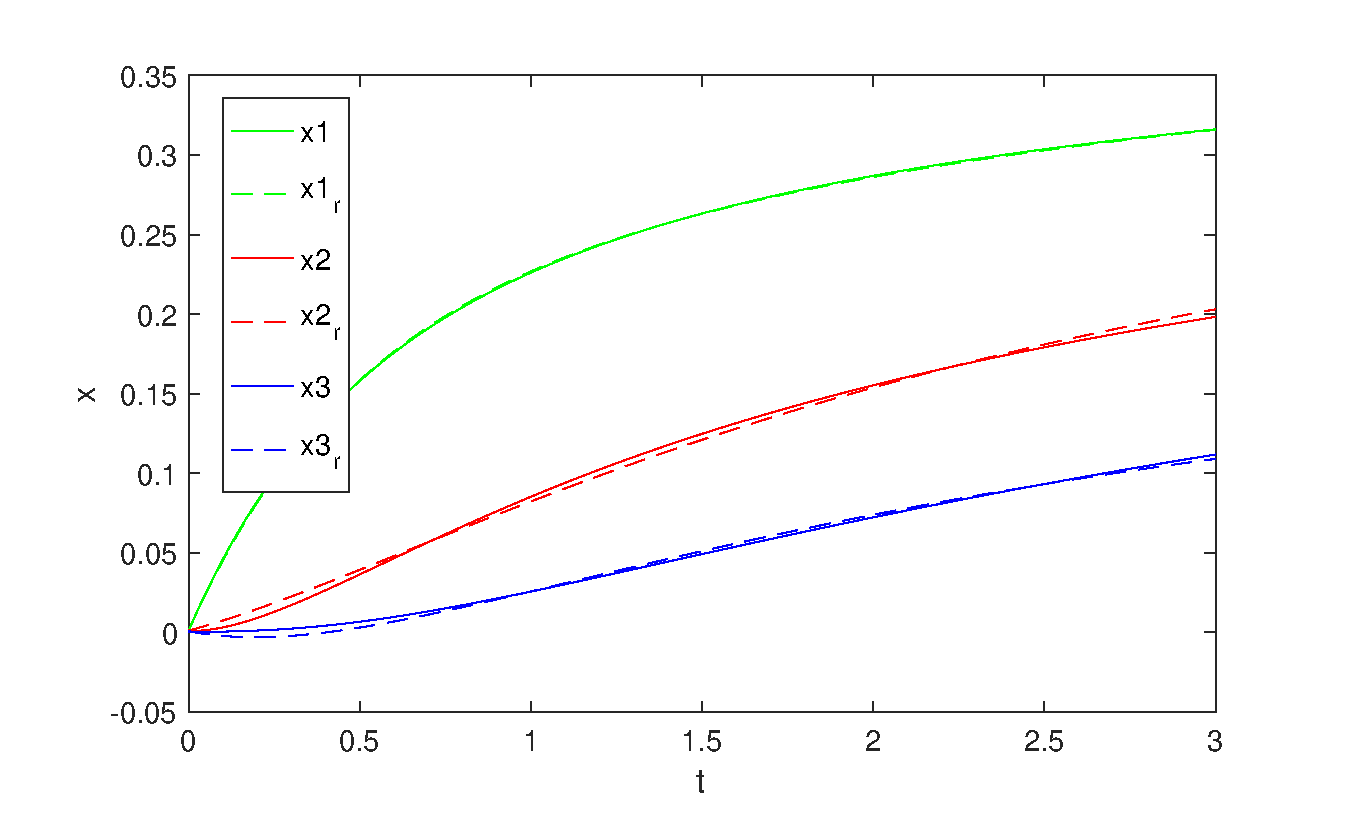
\includegraphics[width=6.5cm]{IC1x_k2comapre.eps}
   \parbox{4cm}{\subcaption{}}
\end{subfigure}%
\begin{subfigure}{.5\textwidth}
  \centering
  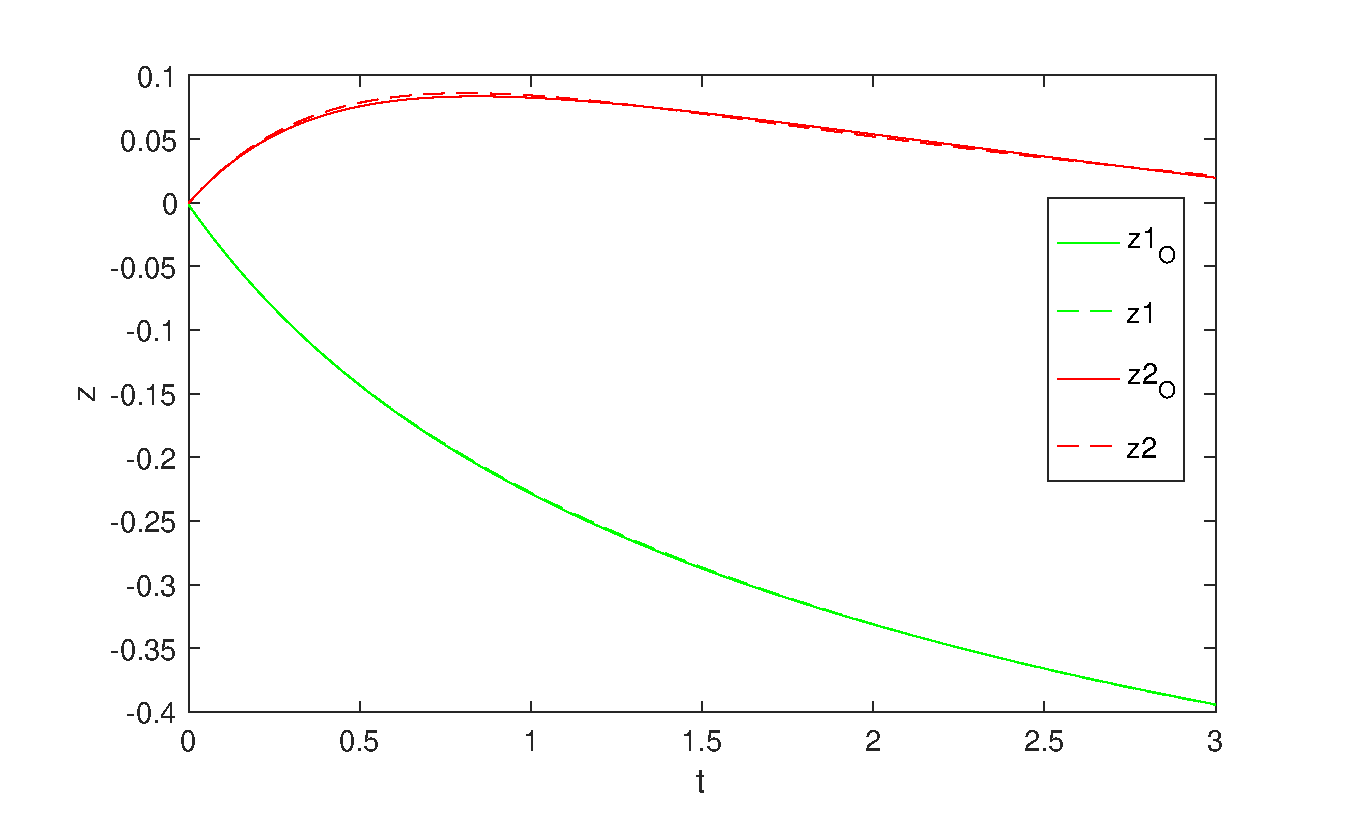
\includegraphics[width=6.5cm]{IC1z_k2comapre.eps}
  \parbox{4cm}{\subcaption{}}
\end{subfigure}
\caption{A nonlinear transmission line circuit model}
\label{fig:sim_IC1}
\end{figure}

\begin{figure}[h]
\begin{subfigure}{.5\textwidth}
  \centering
   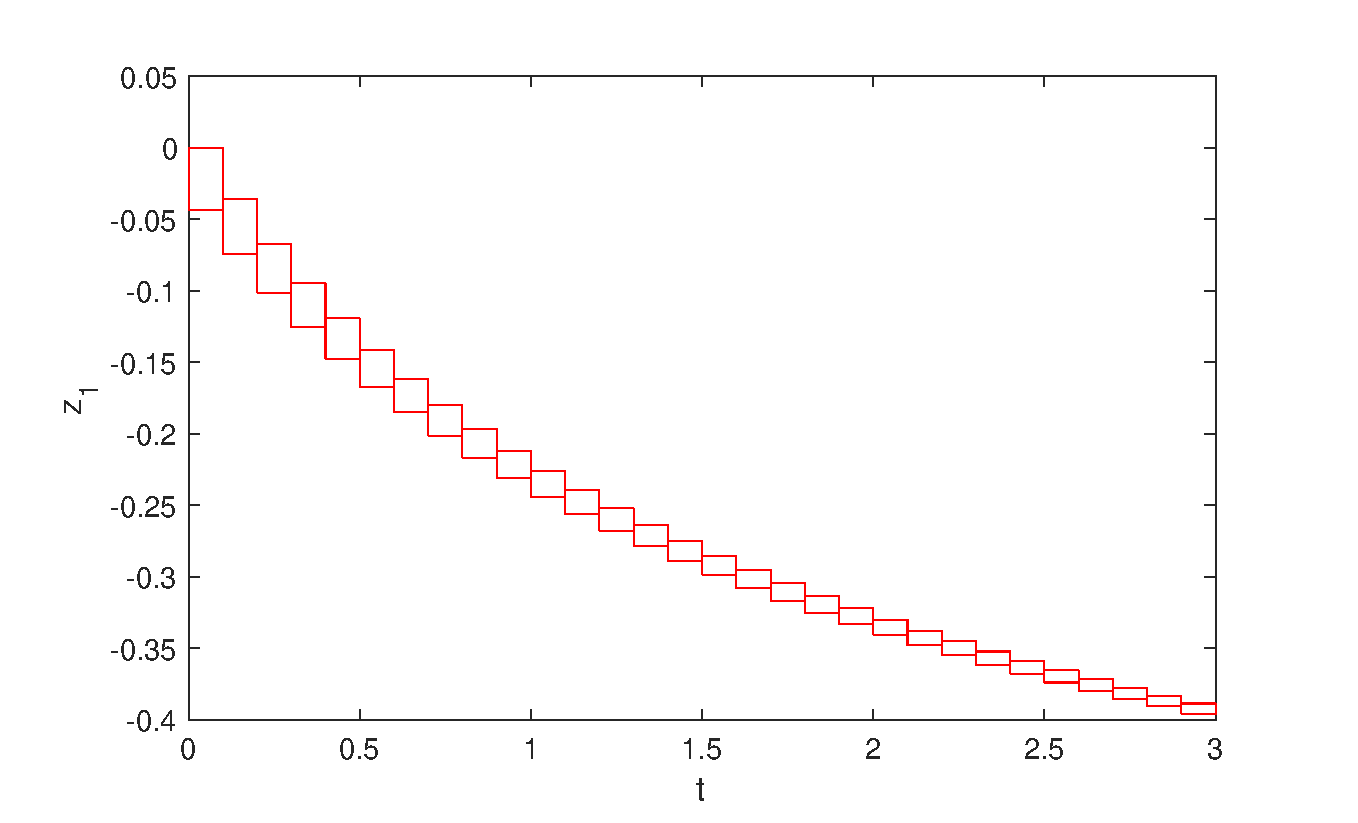
\includegraphics[width=6.5cm]{IC_line_r}
   \parbox{4cm}{\subcaption{}}
\end{subfigure}%
\begin{subfigure}{.5\textwidth}
  \centering
  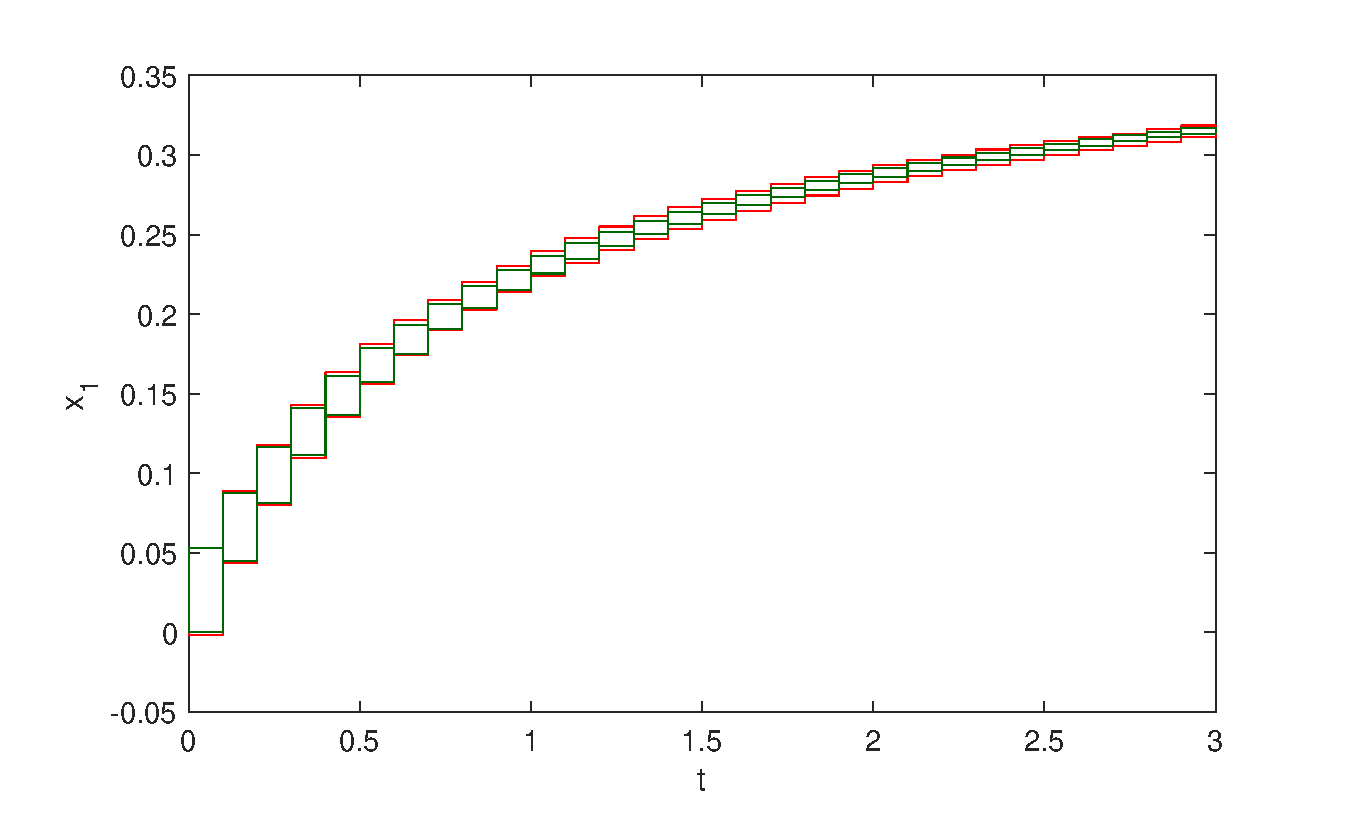
\includegraphics[width=6.5cm]{IC1compare_flowpip.eps}
  \parbox{4cm}{\subcaption{}}
\end{subfigure}%
 \caption{Flow-pipe in a nonlinear transmission line circuit model}
\label{fig:flowpipe_IC1}
\end{figure}


Next circut example is a transmission line circuit model with a quadratic nonlinearity by adding a nonlinear resistor to the ground at each node, and thus the dynamic ODE becomes \cite{REWIENSKI2006426}: 
\begin{align}
\frac{dx}{dt}&=f(x)+Bu,\\
\mbox{with}\quad f(x)&=
\begin{bmatrix}
    -2 & 1 &   &   &  \\
    1  & -2 & 1 &   &  \\
        & \ddots & \ddots & \ddots &  \\
        &    & 1 & -2  & 1\\
        &    &   & 1 & -2
\end{bmatrix} x -
\begin{bmatrix}
    x_1^2  \\
    x_2^2  \\
        \vdots \\
    x_{n-1}^2\\
    x_{n}^2
\end{bmatrix},
\end{align}
where $B=[1,0,\cdots,0]^T$,  input $u=1$, $n=100$, the initial conditional region $X_0=\left\{x \, |\, x_i \in [0,0.0025]  \, \mbox{for}\, i=1\sim20 \wedge x_i=0 \,  \mbox{for}\, i=21\sim100 \right\}$ and $t_f=3$.  In this example, POD method can reduce the dimension to $k=2$.  Figure \ref{fig:sim_IC1} presents that the simulation trajectories are almost overlapped in full-order space (Fig \ref{fig:sim_IC2}(a)) but also in the subspace (Fig \ref{fig:sim_IC2}(b)). Also, the flow-pipe reach set of the original model is included in that of the reduced model in Fig.\ref{fig:flowpipe_IC2}.
\begin{figure}[h]
\begin{subfigure}{.5\textwidth}
  \centering
   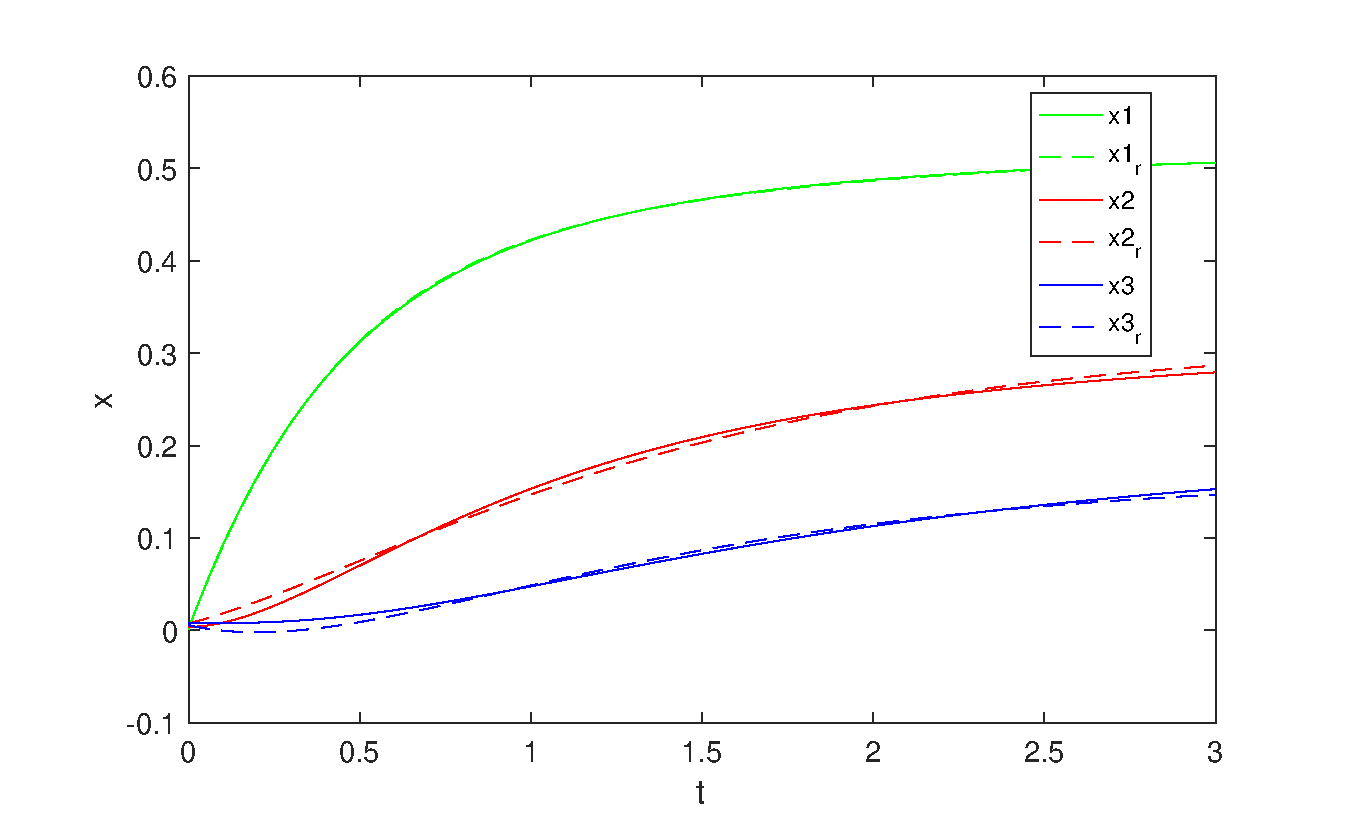
\includegraphics[width=6.5cm]{IC2x_k2comapre.eps}
   \parbox{4cm}{\subcaption{}}
\end{subfigure}%
\begin{subfigure}{.5\textwidth}
  \centering
  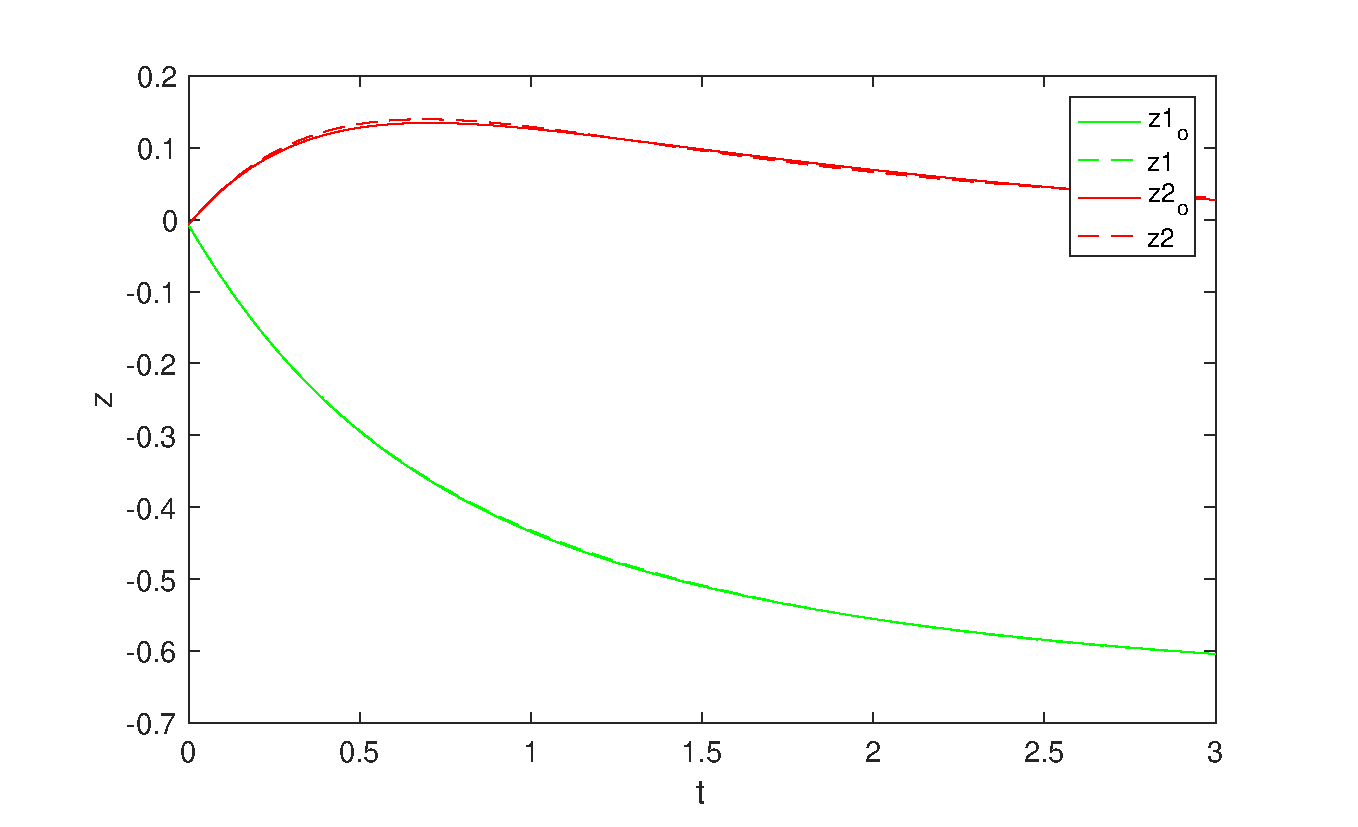
\includegraphics[width=6.5cm]{IC2z_k2comapre.eps}
  \parbox{4cm}{\subcaption{}}
\end{subfigure}
\caption{A nonlinear transmission line circuit model with quadratic nonlinearity}
\label{fig:sim_IC2}
\end{figure}

\begin{figure}[h]
\begin{subfigure}{.5\textwidth}
  \centering
  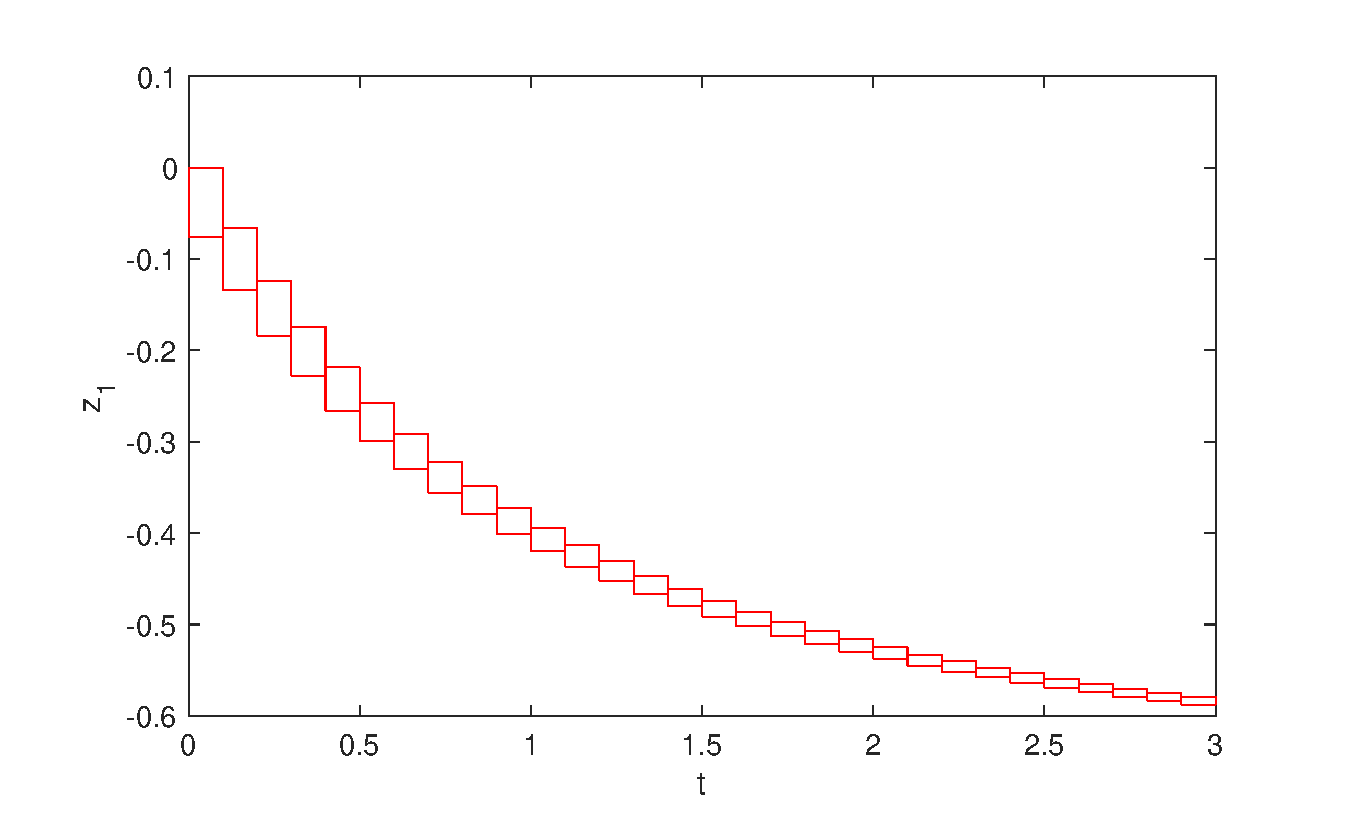
\includegraphics[width=6.5cm]{IC_r.eps}
  \parbox{4cm}{\subcaption{}}
\end{subfigure}%
\begin{subfigure}{.5\textwidth}
  \centering
  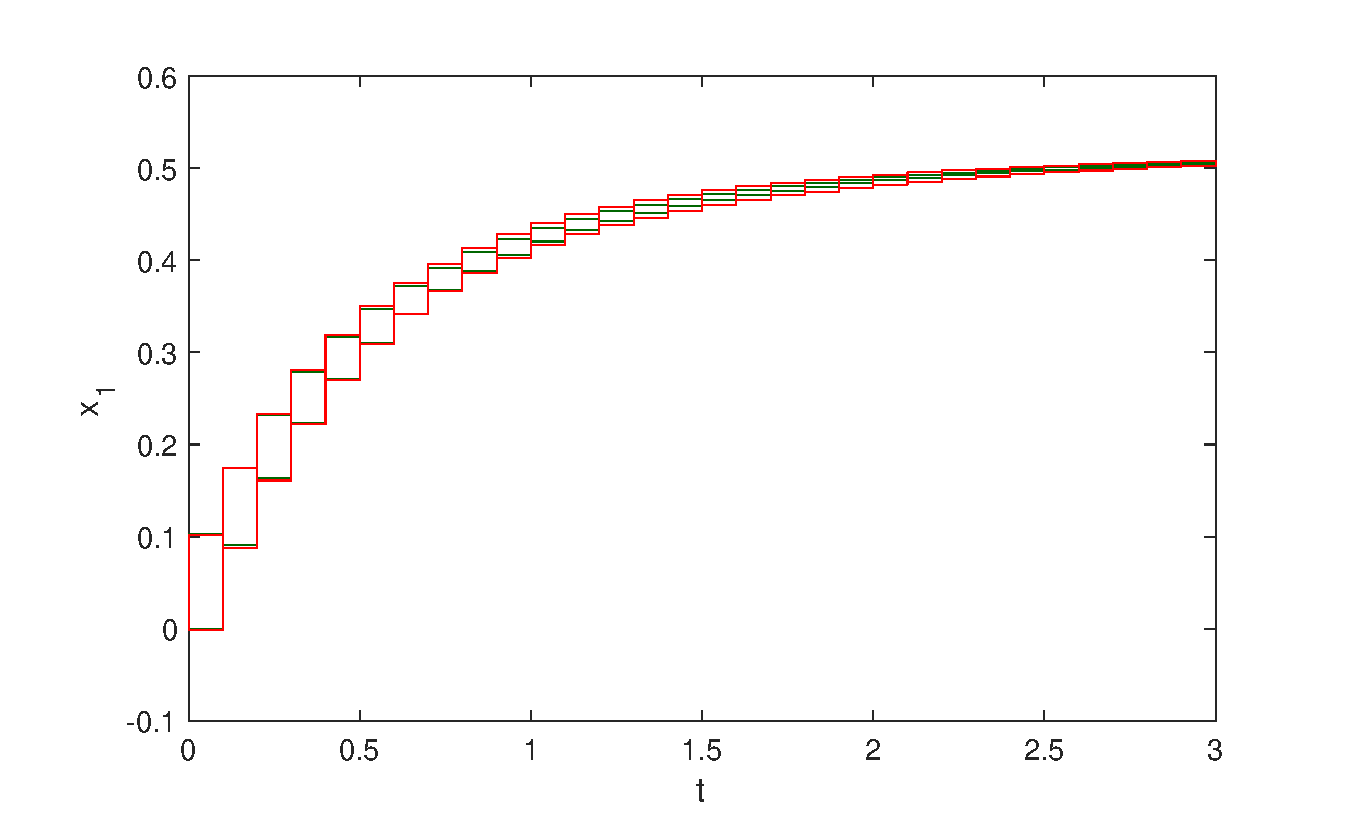
\includegraphics[width=6.5cm]{IC2compare_flowpip.eps}
  \parbox{4cm}{\subcaption{}}
\end{subfigure}%
\caption{Flow-pipe in a quadratic nonlinearity model}
\label{fig:flowpipe_IC2}
\end{figure}

\subsection{Fluid dynamics}
In this study, we also explore a fluid dynamics problem, associated with shock movement in a fluid, which is an inherently nonlinear phenomenon. The fluid dynamics is based on 1D Burgers’ equation, for all $x\in \left[0,l\right]$, $t>0$,
\begin{equation}
\frac{\partial U(x,t)}{\partial t}+\frac{\partial F(U(x,t))}{\partial x}=G(x), \quad \mbox{with}\;U(x,0)=1,\;U(0,t)=u(t),
\end{equation}
where $l$ is the length of the modeled region, $U$ is a conserved quantity (ex. density, heat), $F(U)=0.5U^2$, $G(x)=0.02\exp(0.02x)$, and $u(t)$ is the incoming flow.  After discretizing the partial differential equation with $\bar{U}=\left[U_1, U_2, ...,U_n\right]^T$, where $U_i$ approximates $U$ at point $x_i=i\triangle x$ ($\triangle=l/n$, where n is the number of grid points), we have an n-dimensional ODE equation as bellows \cite{REWIENSKI2006426}:
\begin{align}
\frac{d\bar{U}}{dt}&=f(\bar{U})+Bu,\\
f(\bar{U})&=\frac{1}{\triangle x}
\begin{bmatrix}
    -0.5U_1^2 &  &   &     \\
       & 0.5(U_1^2-U_2^2) &  &     \\
        &  & \ddots &    \\
        &    &  & 0.5(U_{n-1}^2-U_{n}^2)
\end{bmatrix} +
\begin{bmatrix}
    \exp(0.02x_1)     \\
     \exp(0.02x_2)    \\
    \vdots    \\
      \exp(0.02x_n)
\end{bmatrix}
\end{align}
where $B=\left[1/(2\triangle x)0 \cdots0\right]$, and $u=5$ in our study. Also, we consider the initial conditional region $\bar{U}_0=\left\{\bar{U} \, |\, U_i \in [0,0.0025]  \, \mbox{for}\, i=1\sim20 \wedge U_i=0 \,  \mbox{for}\, i=21\sim100 \right\}$ and $t_f=2$.  In this case, the dimension is reduced considerably from $n=100$ to $k=3$.  Simulating the trajectories, there is no obvious difference between that from full-order model and that from reduced-order model, which is shown in Fig. \ref{fig:sim_Fluid}. As we expected, Figure \ref{fig:flowpipe_Fluid} shows the fact that the flow-pipe reach set of the reduced model contain that of the original model.


\begin{figure}[h]
\begin{subfigure}{.5\textwidth}
  \centering
   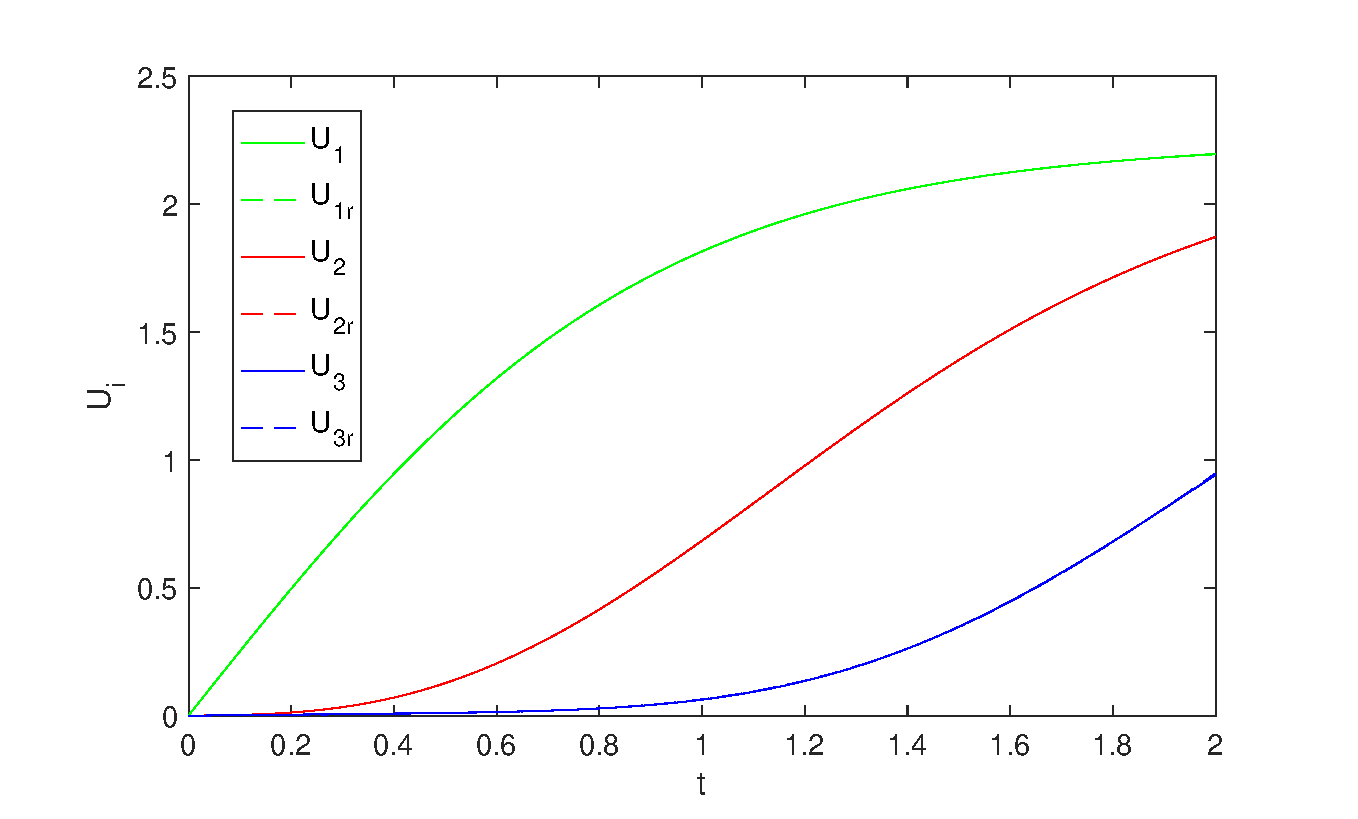
\includegraphics[width=6.5cm]{Fluidcomparek3x.eps}
   \parbox{4cm}{\subcaption{}}
\end{subfigure}%
\begin{subfigure}{.5\textwidth}
  \centering
  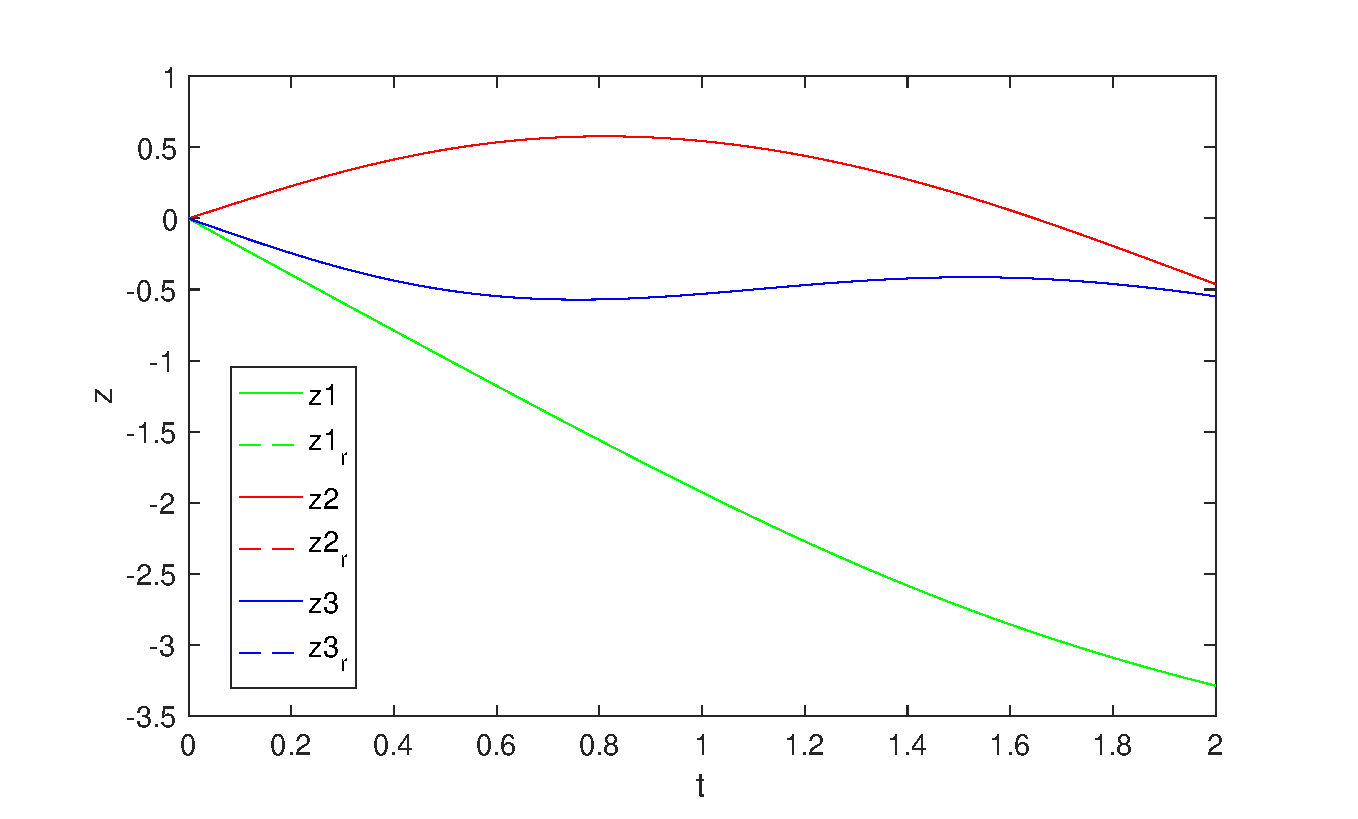
\includegraphics[width=6.5cm]{Fluidcomparek3z.eps}
  \parbox{4cm}{\subcaption{}}
\end{subfigure}
\caption{Fluid dynamic model}
\label{fig:sim_Fluid}
\end{figure}


\begin{figure}[h]
\begin{subfigure}{.5\textwidth}
  \centering
  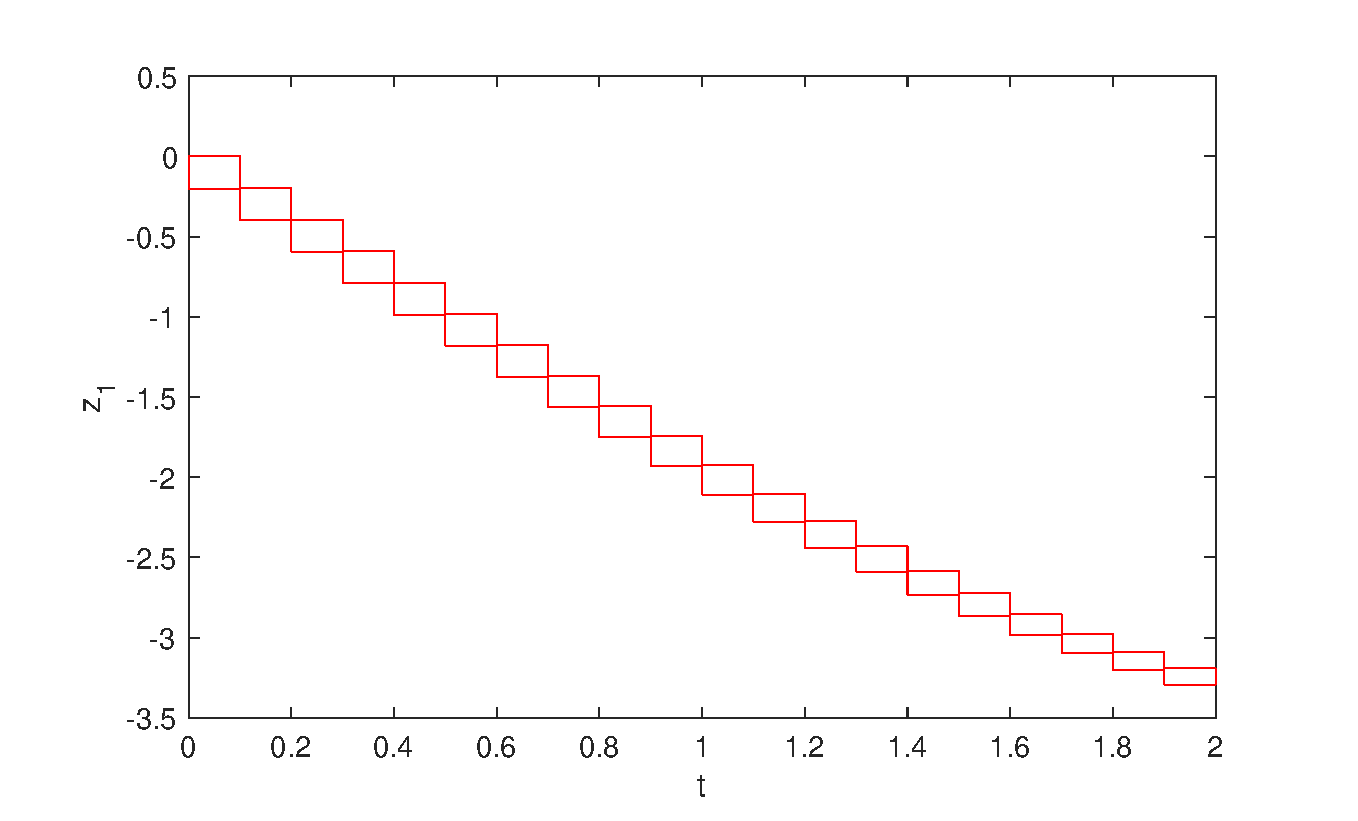
\includegraphics[width=6.5cm]{Fluid_r.eps}
  \parbox{4cm}{\subcaption{}}
\end{subfigure}%
\begin{subfigure}{.5\textwidth}
  \centering
  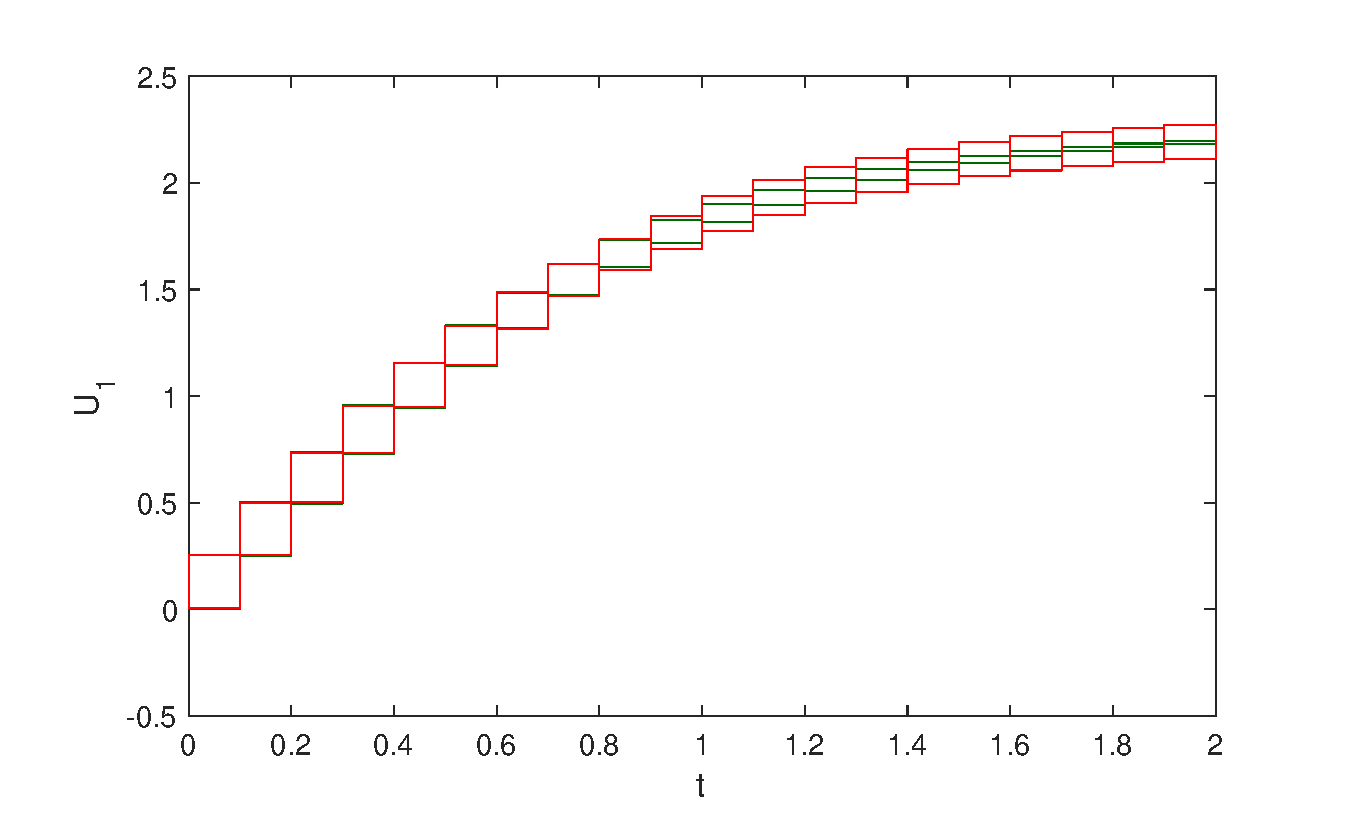
\includegraphics[width=6.5cm]{Fluidflowpipe_compare.eps}
  \parbox{4cm}{\subcaption{}}
\end{subfigure}%
\caption{Flow-pipe in fluid dynamic model}
\label{fig:flowpipe_Fluid}
\end{figure}

\begin{table}[htbp]\scriptsize
  \centering
  \caption{Checking property: For each benchmark, the initial condition region and time region are defined in the subsection of case studies.}
  \label{tab:prop_check}
  \begin{tabular}{ccccc}
    \toprule
    Benchmark & $X_f(S_n)$ & safe & $X_f(S_k)$ & safe\\ \hline
   \multirow{3}{*}{Analog circuits.1($n=100$)} & $x_1\geq 0.35$ & Yes & $U_r(1,1)*z_1 + U_r(1,2)*z_2 \geq 0.33 $& Yes\\
   &$x_2\geq 0.25$ & Yes & $U_r(2,1)*z_1 + U_r(2,2)*z_2 \geq 0.23 $& Yes\\
   &$x_3\geq 0.15$ & Yes & $U_r(3,1)*z_1 + U_r(3,2)*z_2 \geq 0.23 $& Yes\\ \hline
   \multirow{3}{*}{Analog circuits.2($n=100$)} & $x_1\geq 0.6$ & Yes & $U_r(1,1)*z_1 + U_r(1,2)*z_2 \geq 0.566 $& Yes\\
   &$x_2\geq 0.4$ & Yes & $U_r(2,1)*z_1 + U_r(2,2)*z_2 \geq 0.366 $& Yes\\
   &$x_3\geq 0.2$ & Yes & $U_r(3,1)*z_1 + U_r(3,2)*z_2 \geq 0.166 $& Yes\\ \hline
   \multirow{3}{*}{Fluid dynamics($n=100$)} & $x_1\geq 2.5$ & Yes & $U_r(1,1)*z_1 + U_r(1,2)*z_2+U_r(1,3)*z_3 \geq 2.426 $& Yes\\
   &$x_2\geq 2$ & Yes & $U_r(2,1)*z_1 + U_r(2,2)*z_2+U_r(2,3)*z_3 \geq 1.926 $& Yes\\
   &$x_3\geq 1.5$ & Yes & $U_r(3,1)*z_1 + U_r(3,2)*z_2+U_r(3,3)*z_3 \geq 1.426 $& Yes\\ \hline
    \bottomrule
  \end{tabular}
\end{table}

\subsection{Evaluation} 
We experiment those examples by using Matlab 2016b and Flow* on a Mac laptop with 2.4 GHz 64-bit Intel Core i5 and 8GB RAM. For different examples, the corresponding statistical error bound and computation time are given in table\ref{tab:table1}.
It presents that for the models demonstrated previously, running reduced-order systems has improved computation time a lot. Especially, it can still efficiently carry out the problem with very large dimension up to $n=500$, in which running in the original model get timed out.  However, the model of Cellular P53 regulation given in \cite{p53} is a counterexample that simulating in a reduced-order system does always make the computation more efficient. The reason is that even though the dimension is decreased, the number of terms of ODE (the coupling terms between each variable) is increased to keep the same complex information of the system's behavior. As a result, MOR is not always useful for all complicated models. Considering a $n$-dimensional system with $l$-order ODE, its $k$-dimensional reduced system may has the maximal term number $C^{k+l}_l$ for each variable's differential equations. Consequently, to evaluate the total terms of the original system and the reduced system could provide us the idea how it would be efficient to simulate a reduced system. \\
In our trials, MOR method is suitable for a system in which the dynamics of state variables have analogy behavior. Particular for a system arising from discretization of partial differential equations (PDEs), its dimension can be greatly reduced by POD method. The analogy characteristic provides the potential to describe the dynamic of whole system with only few dimensions. We can see that from table\ref{tab:table1}, the analog circuit benchmark and fluid dynamics benchmark coming from discretization of PDE, which has very large dimension, can be described by 5 or less dimension. For the Cellular P53 regulation, the low limit to reduce the dimension significantly occurs from that the most singular values corresponding to singular vectors of the system behavior is not relatively small enough to be ignored in \ref{fig:singular_value} (a). By contrast, the singular values in descending order of fluid dynamic decrease quickly, seen in \ref{fig:singular_value} (b).
 
\begin{table}[htbp]
  \centering
  \caption{The computation time and the statistical error bound corresponding to different benchmarks: n is the dimension of a original system, k is the dimension of a reduced-order abstraction, $|\delta_s|$ is the total statisticalerror bound, OOT represents "out of time" with the time limit = 1 hour. Noted that the minimal reduced dimension $k$ is obtained with a simulation error bound $|e_s|\leq 5 \times 10^{-2}$, , where $|e_s|=\max_t\frac{|x(t)-U_r z(t)|}{|x(t)|}$}
  \label{tab:table1}
  \begin{tabular}{ccccc}
    \toprule
    Benchmark & Time(s) of $S_n$ & $k$ & $|\delta_s| (q=20)$ & Time(s) of $S_k$\\
    \midrule
   Analog circuits.1($n=100$) & 235 & 2 &0.020& 6\\
   Analog circuits.1($n=500$) & OOT & 2 &0.052& 6\\
   Analog circuits.2($n=100$)  & 498 & 2 & 0.034& 0.5\\
   Analog circuits.2($n=500$) & OOT & 2 &0.060& 0.5\\
   Fluid dynamics($n=100$)  & 205 & 3 &0.074&1.4\\
   Fluid dynamics($n=500$)  & OOT& 3 &0.133&2\\
   Cellular P53 regulation($n=6$)  & 110& 4 &51&OOT\\
    \bottomrule
  \end{tabular}
\end{table}

\begin{figure}[h]
\begin{subfigure}{.5\textwidth}
  \centering
  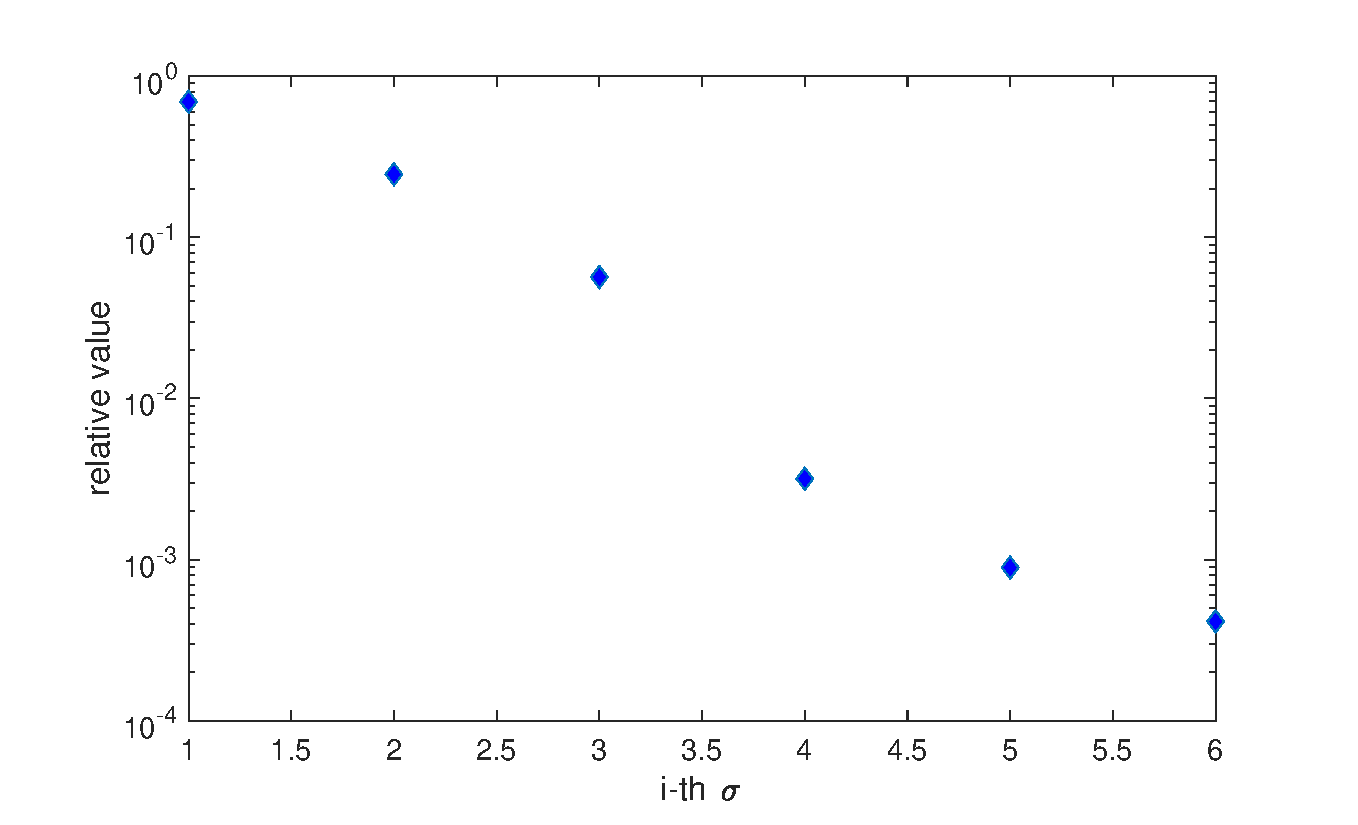
\includegraphics[width=6.5cm]{p53_singular_value_log}
  \parbox{4cm}{\subcaption{}}
\end{subfigure}%
\begin{subfigure}{.5\textwidth}
  \centering
  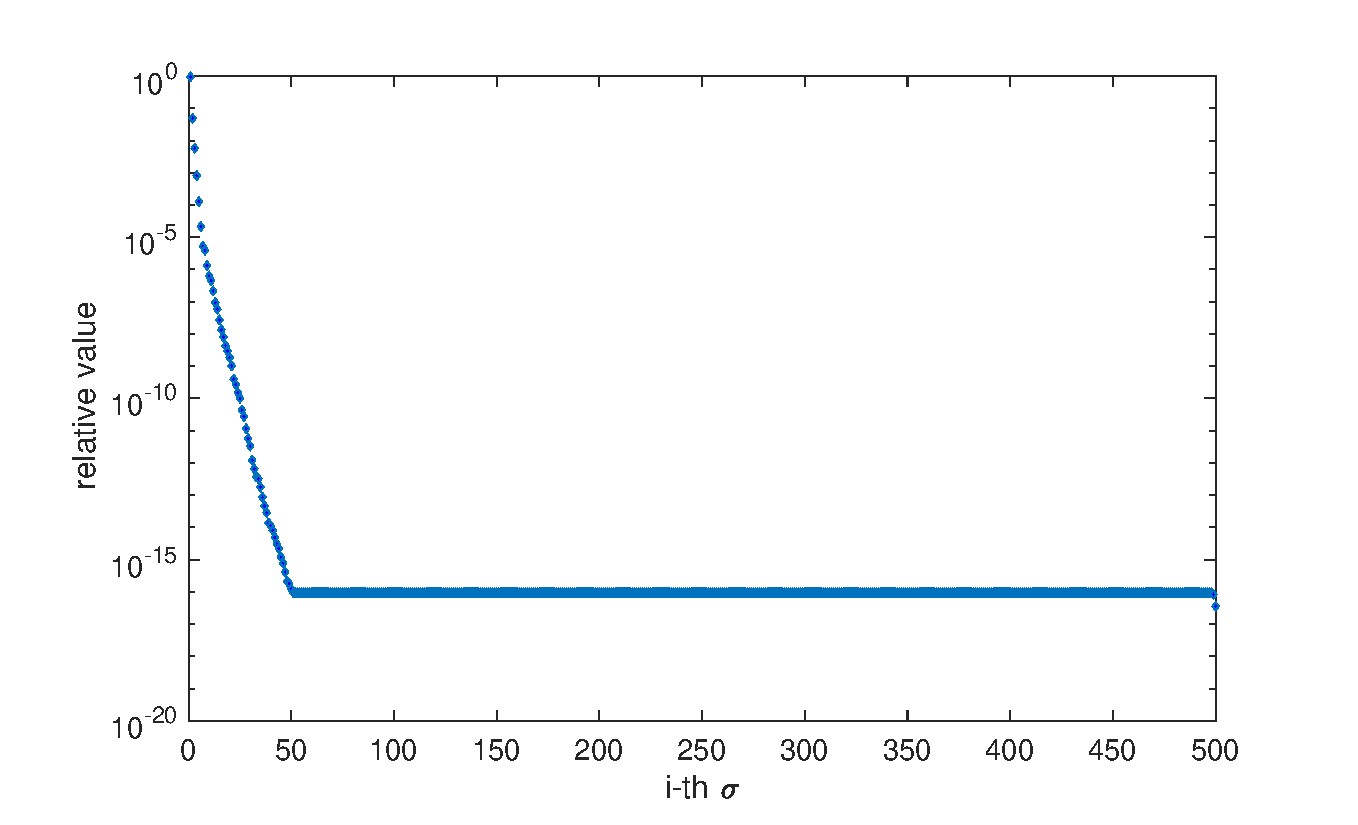
\includegraphics[width=6.5cm]{Fluid_singular_value_log}
  \parbox{4cm}{\subcaption{}}
\end{subfigure}%
\caption{The singular value in descending order: (a) Cellular P53 regulation benchmark. (b) Fluid dynamic benchmark}
\label{fig:singular_value}
\end{figure}

\begin{table}[htbp]\footnotesize
  \centering
  \caption{Varing Initial region of benchmarks: n is the dimension of a original system, k is the dimension of a reduced-order abstraction, $|\delta_s|$ is the total statisticalerror bound, OOT represents "out of time" with the time limit = 1 hour. Noted that the minimal reduced dimension $k$ is obtained with a simulation error bound $|e_s|\leq 5 \times 10^{-2}$.}
  \label{tab:initial_region}
  \begin{tabular}{cccccc}
    \toprule
    Benchmark& Initial set region&Time(s) of& $k$ & $|\delta_s| $ & Time(s) of\\
         &$X_0= \left\{x \, |\, x_i \in [0,b] , \,  1\leq i \leq20;\, \mbox{else} \,x_i=0\right\}$& $S_n$&&(q=20)& $S_k$\\\hline
    \midrule
    Analog circuits.1 & $b=0.0025$ & 235 & 2 &0.020& 6\\
    ($n=100$), $t_f=3$&$b=0.01$ & 241& 2 & 0.1 &7\\
    &$b=0.05$ & 248& 3 & 0.39 &23\\
    &$b=0.1$ & 256& 15 & 0.6 &OOT\\\hline
    Analog circuits.1 & $b=0.0025$&OOT & 2 &0.052& 6\\
    ($n=500$), $t_f=3$&$b=0.01$ & OOT& 2 & 0.17 &7\\
    &$b=0.05$ & OOT& 3 & 0.86 &24\\
    &$b=0.1$ & OOT& 16 & 1.67 &OOT\\\hline
    Analog circuits.2 & $b=0.0025$ & 498 & 2 &0.034& 0.5\\
    ($n=100$), $t_f=3$&$b=0.01$ & 512& 2 & 0.09 &0.5\\
    &$b=0.05$ & 512& 5 & 0.36 &23\\
    &$b=0.1$ & 520& 16 & 0.72 &OOT\\\hline
    Analog circuits.2 & $b=0.0025$&OOT & 2 &0.06& 0.5\\
    ($n=500$), $t_f=3$&$b=0.01$ & OOT& 2 & 0.19 &0.6\\
    &$b=0.05$ & OOT& 5 & 0.84 &23\\
    &$b=0.1$ & OOT& 17 & 1.67 &OOT\\\hline
    Fluid dynamics & $b=0.0025$ & 205 & 3 &0.074&1.4\\
    ($n=100$), $t_f=2$ &$b=0.01$ & 229& 3 & 0.22 &1.5\\
    &$b=0.05$ & 227& 5 & 0.98 &14.8\\
    &$b=0.1$ & 257& 18 & 2.0 &OOT\\\hline
    Fluid dynamics & $b=0.0025$&OOT & 3 &0.133&2\\
    ($n=500$), $t_f=2$ &$b=0.01$ & OOT& 3 & 2.5 &2.3\\
    &$b=0.05$ & OOT& 10 & 2.5 &OOT\\
    &$b=0.1$ & OOT& 17 & 4.68 &OOT\\\hline
    \bottomrule
  \end{tabular}
\end{table}

 \begin{table}[htbp]\footnotesize
  \centering
  \caption{Varing time region of benchmarks with a fixed parameter $b=0.01$ of the initial condition region.}
  \label{tab:time_region}
  \begin{tabular}{cccccc}
    \toprule
    Benchmark& $t_f$ &Time(s) of& $k$ & $|\delta_s| $ & Time(s) of\\
         && $S_n$&&(q=20)& $S_k$\\\hline
    \midrule
    Analog circuits.1 & 1 & 31 & 2 &0.1& 2\\
    ($n=100$)&3 & 241& 2 & 0.1 &7\\
    &6 & 1033& 2 & 0.32 &15\\
    &12 & OOT& 2 & 0.34 &33\\
    &20 & OOT& 3 & 0.23 &160\\\hline
    Analog circuits.1 & 1 & OOT & 2 &0.16& 2\\
    ($n=500$)&3 & OOT& 2 & 0.17 &7\\
    &6 & OOT& 2 & 0.58 &15\\
    &12 &OOT& 2 & 0.60 &33\\
    &20 & OOT& 3 & 0.31 &100\\\hline
    Analog circuits.2 & 1 & 114 & 2 &0.09& 0.3\\
    ($n=100$)&3 &512 & 2 & 0.09 &0.5\\
    &6 & 1761& 2 & 0.09 &1\\
    &12 & OOT& 2 & 0.19 &2\\
    &20 & OOT& 3 & 0.2 &13\\\hline
    Analog circuits.2 & 1 & OOT & 2 &0.19& 0.3\\
    ($n=500$)&3 & OOT& 2 & 0.19 &0.6\\
    &6 & OOT& 2 & 0.21 &1\\
    &12 &OOT& 2 & 0.21 &2\\
    &20 & OOT& 3 & 0.52 &13\\\hline
    Fluid dynamics & 1 & 113 & 2 &0.24& 0.3\\
    ($n=100$)&2 & 229& 3 & 0.22 &1.5\\
    &4 & 1584& 5 & 0.21 &64\\
    &8 & OOT& 8 & 2.77 &1920\\\hline
    Fluid dynamics & 1 & OOT & 3 &0.91 & 1.4\\
    ($n=500$)&2 & OOT& 3 & 2.5 &2.3\\
    &4 & OOT& 5 & 0.53 &64\\
    &8 & OOT& 8 & 0.52 &2621\\\hline
    \bottomrule
  \end{tabular}
\end{table}

Now, we analyze the applicability of MOR method in those benchmarks by increasing the initial condition region. According to Table \ref{tab:initial_region}, it has shown that MOR method is no longer suitable when the variance raises to $0.1$. In that initial condition region, the minimal $k$ is large to ten digits, which is accompanied by a very large number of terms of ODE. Consequently, computing in reduced system becomes less efficient than in original system. Also, the statistical error bound is too large as the variance increase to $0.05$, and thus verification of reduced model is meaningless in this condition.

Furthermore, let's consider the statistical error bound related to the time duration. Table \ref{tab:time_region} presents that as  $t_f$ increases, the error bound increase to a noticeably number. To alleviate this problem, one may decrease the error bound by increasing $k$, but that will cause a dramatic growing in the number of terms of ODE. Therefore, using MOR method involves a trade-off between the reduced dimension $k$ and the error bound.

\section{Conclusion and future work}  \label{conclusion}
We proposed a method to carry out the statistical verification of safe properties in large-dimensional non-linear systems efficiently. Also, we implemented it in some benchmarks, and the computation time in the verification process is significantly decreased with the MOR. Here, the reachability problem is discussed with a statistical property. To extend the practice, we may explore the falsification of a reduced abstraction, which could guide us to find a counter-example in an original system.
\bibliographystyle{Science}
\bibliography{typeinst}





\end{document}
